\documentclass{article}
\usepackage{algorithm}
\usepackage{algpseudocode}
\usepackage{amsmath}
\usepackage{amssymb}
\usepackage{amsthm}
\usepackage[titletoc]{appendix}
\usepackage{array}
\usepackage[english]{babel}
\usepackage{booktabs}
\usepackage{cancel}
\usepackage{color}
\usepackage{eqparbox}
\usepackage{float}
\usepackage[margin=1in]{geometry}
\usepackage{graphicx}
\usepackage[hidelinks]{hyperref}
% *must* be loaded after hyperref
\usepackage[toc, acronym, numberedsection=nameref]{glossaries}
\usepackage[utf8]{inputenc}
\usepackage{lipsum}
\usepackage{mathtools}
\usepackage[cache=false]{minted}
\usepackage{parskip}
\usepackage{pgfplots}
\usepackage{scalerel}
\usepackage{skull}
\usepackage{subcaption}
\usepackage{titling}
\usepackage{textcomp}
\usepackage{tikz}
\usepackage[compact, explicit]{titlesec}
\usepackage{textcomp}
\usepackage[nottoc]{tocbibind}
\usepackage[textsize=small]{todonotes}
\usepackage[normalem]{ulem}

% Document Settings

\definecolor{__minted_background_color}{rgb}{0.95, 0.95, 0.98}
\definecolor{__minted_highlight_color}{rgb}{0.88, 0.88, 1.0}
\setminted{autogobble=true,
           style=tango,
           breaklines,
           bgcolor=__minted_background_color,
           highlightcolor=__minted_highlight_color,
           mathescape, % Escape math mode everywhere.
           texcomments,  % Enable latex code inside of comments. Useful for referencing equations.
    }

\usetikzlibrary{arrows, automata, shapes, positioning}
\pgfplotsset{compat=1.16}
\numberwithin{equation}{section}
% Sets the width of the margin TODO notes
\setlength{\marginparwidth}{0.84in}
\reversemarginpar{}

% hex #184c9a
\definecolor{__glossary_entry_color}{rgb}{0.094, 0.298, 0.604}
\renewcommand{\glstextformat}[1]{\textbf{\textcolor{__glossary_entry_color}{#1}}}

% Add glos: to the beginning of the glossary labels.
\renewcommand*{\glsautoprefix}{glos:}

% All I want is to have comment italicized, but I cant figure out how
% to properly modify the existing \Comment macro.
% \algrenewcomment[1]{\hfill\eqparbox{COMMENT}{\textit{// #1}}}
\algnewcommand{\IComment}[1]{\Comment{\textit{#1}}}

% TODO: Should this path be relative to the document root or this file?
\graphicspath{{./figures/}}

% Document Definitions

\newcommand{\C}{\mathbb{C}}
\newcommand{\R}{\mathbb{R}}
\newcommand{\Z}{\mathbb{Z}}
\newcommand{\N}{\mathbb{N}}
\renewcommand{\O}{\mathcal{O}}

\theoremstyle{definition}
\newtheorem{defn}{Definition}[section]

\theoremstyle{plain}
\newtheorem{thm}{Theorem}[section]

\renewcommand{\qedsymbol}{$\skull$}

% An inline TODO command. Doesn't play nicely with \todotableofcontents
\newcommand\todoinline[2][]{\todo[inline, caption={TODO}, #1]{
\begin{minipage}{\textwidth-4pt}#2\end{minipage}}}

% Draw clouds around things. Useful in mathematical proofs.
\newcommand{\cloud}[4][\dots]{%
    \raisebox{-0.4\height}{%
        \begin{tikzpicture}
            \node [cloud,
                   draw,
                   cloud puffs=#2,
                   cloud ignores aspect,
                   minimum height=#3,
                   minimum width=#4] {#1};
        \end{tikzpicture}
    }
}

% Use \ceil*{} or \floor*{}
\DeclarePairedDelimiter{\ceil}{\lceil}{\rceil}
\DeclarePairedDelimiter{\floor}{\lfloor}{\rfloor}

\AtBeginDocument{%
\renewcommand{\sectionautorefname}{Problem}
}

% make each \section a problem.
\titleformat{\section}[runin]{\large\bfseries}{}{0pt}{\titlerule[1.5pt]\newline\vspace*{-4pt}
Problem\quad\thesection\newline}[\vspace{0.01ex}{\titlerule[1.5pt]}]


\title{Homework 3}
\author{Austin Gill}
\date{March 25, 2019}

\begin{document}
\maketitle

\section{}
\begin{quote}
    Eliminate $B$ from the grammar with production rules
    \begin{align*}
        S & \to aSB \mid bB \\
        B & \to aA \mid b
    \end{align*}
\end{quote}

The variable $B$ may be eliminated from the grammar by substituting the productions $B \to aA \mid b$ wherever $B$ is used in another production rule.
Thus we have\footnote{What should I do with the variable $A$?}
\begin{align*}
    S & \to aSaA \mid aSb \mid baA \mid bb \\
    A & \to \cloud[??]{9}{0.5cm}{0.5cm}
\end{align*}

\section{}
\begin{quote}
    Transform the grammar with production rules
    \begin{align*}
        S & \to aSaa \mid A \\
        A & \to abA \mid bb
    \end{align*}
    into Chomsky normal form.
\end{quote}

\begin{defn}
    A context-free grammar is in Chomsky normal form is all productions are of the form \[A \to BC\] or \[A \to a\] where $A$, $B$, and $C$ are variables, and $a$ is a terminal symbol.
\end{defn}

Our approach will be to use the algorithm given in the proof of Theorem 6.6.
\begin{quote}
    Construct a new, equivalent grammar $G_1$ from $G$ by considering all productions of the form
    \[A \to x_1 x_2 \cdots x_n\]
    If $n = 1$, then $x_1$ must be a terminal symbol since we have, by assumptions, removed all unit productions.
    In this case, ($A \to x_1 \in T$) put the production into $P_1$.
    In cases where $n \geq 2$, introduce a new variable $B_a$ for each $a \in T$.
    Then for each production above, put into $P_1$ the production
    \[A \to C_1 C_2 \cdots C_n\]
    where
    \[C_i = \begin{cases}
            x_i & \text{if $x_i \in V$} \\
            B_a & \text{if $x_i = a$}
        \end{cases}\]
    Then for each variable $B_a$, put into $P_1$ the production \[B_a \to a\]

    We then introduce additional variables necessary to trim production rules of the form
    \[A \to B_1 B_2 \cdots B_n\]
    to a collection of rules of the form \[A \to B_1 B_2\]

    The resulting grammar will be in Chomsky normal form.
\end{quote}

Then for the problem at hand, the algorithm requires a grammar without unit productions, so we remove the production $S \to A$
\begin{align*}
    S & \to aSaa \mid abA \mid bb \\
    S & \to abA \mid bb
\end{align*}
and proceed with the first step of the algorithm.
This yields the productions
\begin{align*}
    S   & \to B_a S B_a B_a \mid B_a B_b A \mid B_b B_b \\
    A   & \to B_a B_b A \mid B_b B_b                    \\
    B_a & \to a                                         \\
    B_b & \to b
\end{align*}
Then we apply the second step to trim each production resulting in a sequence of variables.
\begin{align*}
    S   & \to B_a D_1 \\
    D_1 & \to S D_2   \\
    D_2 & \to B_a B_a \\
    S   & \to B_a D_3 \\
    D_3 & \to B_b A   \\
    S   & \to B_b B_b \\
    A   & \to B_a D_4 \\
    D_4 & \to B_b a   \\
    A   & \to B_b B_b \\
    B_a & \to a       \\
    B_b & \to b
\end{align*}
Which can be more succinctly written as
\begin{align*}
    S   & \to B_a D_1 \mid B_a D_3 \mid B_b B_b \\
    A   & \to B_a D_4 \mid B_b B_b              \\
    D_1 & \to S D_2                             \\
    D_2 & \to B_a B_a                           \\
    D_3 & \to B_b A                             \\
    D_4 & \to B_b a                             \\
    B_a & \to a                                 \\
    B_b & \to b
\end{align*}

\section{}
\begin{quote}
    Transform the following grammar into Chomsky normal form.
    \begin{align*}
        S & \to aSb \mid b
    \end{align*}
\end{quote}

The above process can be repeated to get the productions
\begin{align*}
    S   & \to B_a S B_b \mid b \\
    B_a & \to a                \\
    B_b & \to b
\end{align*}
which can be expanded to
\begin{align*}
    S   & \to B_a C_1 \mid b \\
    C_1 & \to S B_b          \\\
    B_a & \to a              \\
    B_b & \to b
\end{align*}

\section{}
\begin{quote}
    Find a context free grammar for the language of all palindromes with the alphabet $\Sigma = \{a, b\}$.
\end{quote}

Consider $S \to aSa \mid bSb \mid \lambda$.
This set of production rules generates all even-length palindromes.
It's a simple change to allow odd-length palindromes --- simply add $S \to a$ and $S \to b$.
Then we're left with the productions
\[S \to aSa \mid bSb \mid a \mid b \mid \lambda \]

\section{}
\begin{quote}
    Remove all unit-productions, useless productions, and $\lambda$-productions from the grammar with production rules
    \begin{align*}
        S & \to aA \mid aBB      \\
        A & \to aaA \mid \lambda \\
        B & \to bB \mid bbC      \\
        C & \to B
    \end{align*}
\end{quote}

We can remove undesirable productions in the order
\begin{enumerate}
    \item Remove $\lambda$-productions
    \item Remove unit-productions
    \item Remove useless productions
\end{enumerate}

First, consider the following example
\begin{quote}
    Remove $\lambda$-productions from the productions
    \begin{align*}
        S & \to aA             \\
        A & \to a \mid \lambda
    \end{align*}
    We simply replace every occurrence of $A$ with its possible values.
    \begin{align*}
        S & \to aA \mid a \\
        A & \to a
    \end{align*}
    Now consider the productions
    \begin{align*}
        S & \to aA              \\
        A & \to aA \mid \lambda
    \end{align*}
    Here, we have
    \begin{align*}
        S & \to aA \mid a \\
        A & \to aA \mid a
    \end{align*}
\end{quote}
Returning to the problem at hand, removing the $\lambda$-productions from the productions
\begin{align*}
    S & \to aA \mid aBB      \\
    A & \to aaA \mid \lambda \\
    B & \to bB \mid bbC      \\
    C & \to B
\end{align*}
yields
\begin{align*}
    S & \to aA \mid a \mid aBB \\
    A & \to aaA \mid aa        \\
    B & \to bB \mid bbC        \\
    C & \to B
\end{align*}

We then remove the unit-production $C \to B$ to get
\begin{align*}
    S & \to aA \mid a \mid aBB \\
    A & \to aaA \mid aa        \\
    B & \to bB \mid bbB        \\
    C & \to B
\end{align*}
and remove the now-useless production $C \to B$ to get the final simplified production rules.
\begin{align*}
    S & \to aA \mid a \mid aBB \\
    A & \to aaA \mid aa        \\
    B & \to bB \mid bbB
\end{align*}

\section{}
\begin{quote}
    Convert the grammar with productions
    \begin{align*}
        S & \to AB \mid aB       \\
        A & \to abb \mid \lambda \\
        B & \to bbA
    \end{align*}
    into Chomsky normal form, and draw the dependency graph for the grammar.
\end{quote}

Before we can convert the productions into Chomsky normal form, we must simplify them according to the processes above.

First, we remove the $\lambda$-production $A \to \lambda$:
\begin{align*}
    S & \to AB \mid B \mid aB \\
    A & \to abb               \\
    B & \to bbA \mid bb
\end{align*}
Second, we remove the unit-production $S \to B$:
\begin{align*}
    S & \to AB \mid bbA \mid bb \mid aB \\
    A & \to abb                         \\
    B & \to bbA \mid bb
\end{align*}
Third, we remove look for useless productions and find none.

We can now proceed to convert the now simplified productions into Chomsky normal form.
So we apply the first step of the algorithm, which yields
\begin{align*}
    S   & \to AB \mid B_b B_b A \mid B_b B_b \mid B_a B \\
    A   & \to B_a B_b B_b                               \\
    B   & \to B_b B_b A \mid B_b B_b                    \\
    B_a & \to a                                         \\
    B_b & \to b
\end{align*}
Then we apply the second step to trim each of the productions that are too large.
This yields
\begin{align*}
    S   & \to AB \mid B_b C_1 \mid B_b B_b \mid B_a B \\
    C_1 & \to B_b A                                   \\
    A   & \to B_a C_2                                 \\
    C_2 & \to B_b B_b                                 \\
    B   & \to B_b C_3 \mid B_b B_b                    \\
    C_3 & \to B_b A                                   \\
    B_a & \to a                                       \\
    B_b & \to b
\end{align*}
which are the simplified production rules in Chomsky normal form.

\begin{figure}[h]
    \centering
    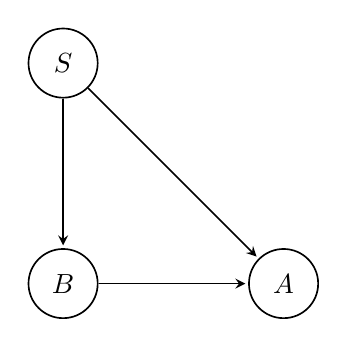
\begin{tikzpicture}[
            ->,
            > = stealth,
            shorten > = 1pt,
            auto,
            node distance = 2.8cm,
            on grid,
            semithick
        ]
        \node[state] (S) {$S$};
        \node[state, below of=S] (B) {$B$};
        \node[state, right of=B] (A) {$A$};

        \path (S) edge (A);
        \path (S) edge (B);
        \path (B) edge (A);
    \end{tikzpicture}
    \caption{The dependency graph before normalization}\label{fig:dep-graph}
\end{figure}

The dependency graph for the grammar before the normalization is shown in \autoref{fig:dep-graph}.
Compare this with the dependency graph for the grammar after the normalization shown in \autoref{fig:dep-graph-fuck}.

\begin{figure}[h]
    \centering
    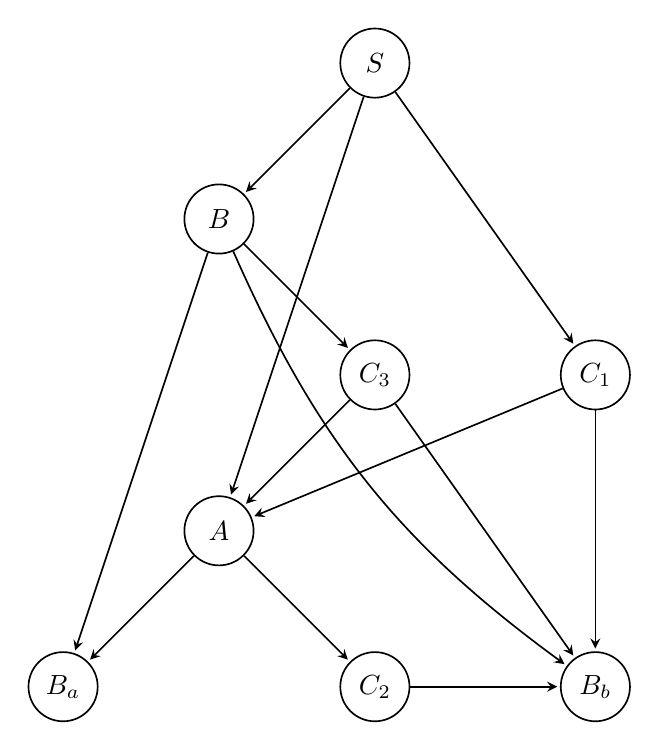
\begin{tikzpicture}[
            ->,
            > = stealth,
            shorten > = 1pt,
            auto,
            node distance = 2.8cm,
            on grid,
            semithick
        ]
        \node[state] (S) {$S$};
        \node[state, below left of=S] (B) {$B$};
        \node[state, below right of=B] (C3) {$C_3$};
        \node[state, right of=C3] (C1) {$C_1$};
        \node[state, below left of=C3] (A) {$A$};
        \node[state, below left of=A] (Ba) {$B_a$};
        \node[state, below right of=A] (C2) {$C_2$};
        \node[state, right of=C2] (Bb) {$B_b$};

        \path (S) edge (C1);
        \path (S) edge (A);
        \path (S) edge (B);
        \path (A) edge (C2);
        \path (A) edge (Ba);
        \path (B) edge (C3);
        \path (B) edge (Ba);
        \path (B) edge[bend right=15] (Bb);
        \path (C1) edge (Bb);
        \path (C1) edge (A);
        \path (C2) edge (Bb);
        \path (C3) edge (Bb);
        \path (C3) edge (A);
    \end{tikzpicture}
    \caption{The dependency graph after normalization}\label{fig:dep-graph-fuck}
\end{figure}

\section{}
\begin{quote}
    Use the pumping lemma for context-free grammars to show that the language $L = \{a^p \mid p \text{ prime}\}$ is not context-free.\todo{Hint: Let $z = a^p = uvwxy$ with $p > m$.}

\end{quote}

\begin{lemma}
    Let $L$ be an infinite context-free language.
    Then there is an $m \in \Z_+$ such that for all $w \in L$ with $\vert w \vert \geq m$, $w$ can be written in the form $w = uvxyz$ where the following properties hold.
    \begin{align*}
        \vert vy \vert  & \geq 1                    \\
        \vert vxy \vert & \leq m                    \\
        u v^k x y^k z   & \in L  & \forall k \geq 0
    \end{align*}
\end{lemma}

This was a problem I used before the last exam to study the pumping lemma for regular languages.
So I include two proofs --- one that the language $L$ cannot be regular --- and one that $L$ cannot be context-free.
However, note that a nonregular language \textit{can} be context-free.
Thus the first proof is not sufficient.

\begin{proof}
    We wish to show that $L = \{a^p \mid p \text{ prime}\}$ is not regular.
    So suppose by way of contradiction that $L$ \textit{is} regular.
    Then the pumping lemma for infinite regular languages holds for some $m$.

    Now consider $w \in L$ given by $w = a^{m + r}$.
    Then $w$ can be decomposed into
    \begin{align*}
        w & = xyz                                                                               \\
          & = \underbrace{\overbrace{a \cdots a}^m}_{xy}\underbrace{\overbrace{a \cdots a}^r}_z \\
          & = a^{m - k} a^k a^r
    \end{align*}
    where $y = a^k$.

    But now consider\footnote{Coming up with the right value for $i$ took several hours along with several pages of failed attempts.} $w_i = xy^i z$ where $i = m + r + 1$
    \begin{align*}
        w_i & = xy^i z                         \\
            & = a^{m - k} {(a^k)}^i a^r        \\
            & = a^{m - k} a^{k(m + r + 1)} a^r \\
            & = a^{(k + 1)(m + r)}
    \end{align*}
    which is \textit{not} in $L$, because $(k + 1)(m + r)$ is clearly\texttrademark{} not prime.
    This is a contradiction, and thus $L$ is not regular.
\end{proof}

However, as noted above, showing that a language is not regular does not imply that it is context-free.
The proof above is worked through in order to inspire the following proof.

\begin{proof}
    We wish to show that $L = \{a^p \mid p \text{ prime}\}$ is not context-free.
    So suppose by way of contradiction that $L$ \textit{is} context-free.
    Then the Pumping Lemma for infinite context-free languages holds for some $m$.

    So consider some $w \in L$ given by $w = a^p$, where $p \geq m$ is prime.
    \begin{align*}
        w & = a^p   \\
          & = uvxyz
    \end{align*}
    with $\vert vy \vert \geq 1$, and $\vert vxy \vert \leq m$.
    Note also that $\vert w \vert = p$.

    How consider $w_i = u v^i x y^i z$ with $i = p + 1$.
    \begin{align*}
        w_i & = u v^{p + 1} x y^{p + 1} z \\
            & = u v v^p x y y^p z
    \end{align*}
    but then
    \begin{align*}
        \vert w_i \vert & = \vert u v v^p x y y^p z \vert                     \\
                        & = \vert w \vert + \vert v^p \vert + \vert y^p \vert \\
                        & = p + p + p                                         \\
                        & = 3p
    \end{align*}
    Thus $w_i \notin L$, because $3p$ is not prime.
    This is a contradiction, and therefore $L$ cannot be context-free.
\end{proof}
\end{document}
